\chapter{Evaluation}
In this chapter, the tool will be put in to test with two computational model, influenza1918 and Covasim. Influenza1918 is a relatively simple model compare to Covasim, this chapter will go through the testing process more both model, and the result produced, then some discussion about the result.
\section{Testing influenza1918}
Influenza1918 is an equation-based model originally developed to for the need to design model validation strategies, this is a model that simulate epidemiological disease-spread of the course of the 1918 Influenza epidemic within the United States.
This model has five state variables and six parameters \cite{Reference24}.
\subsection{Testing process for influenza1918}
First, a scenario name influenza1918 is created, by creating this scenario, the basic files for testing is also auto generated. Since influenza1918 is implemented through OpenModelica in a \textsl{influenza1918.mo} file, so to test this model, first user need to put the model file into the \textsl{\textbackslash scenarios\textbackslash influenza1918 \textbackslash model}. Next use the “Edit dot files” button to start edit the relations of the parameters. A file named influenza1918\_abstract is created, there are two graph needed, first is \textsl{cluster\_inputs} with the input parameters, then \textsl{cluster\_outputs} with the output parameters. In the right panel, enter the file name influenza1918\_abstract, then select the type of graph, input the graph name and label, and the parameters for the selected cluster, click add graph to apply the change.
\begin{figure}[H]
	\centering
	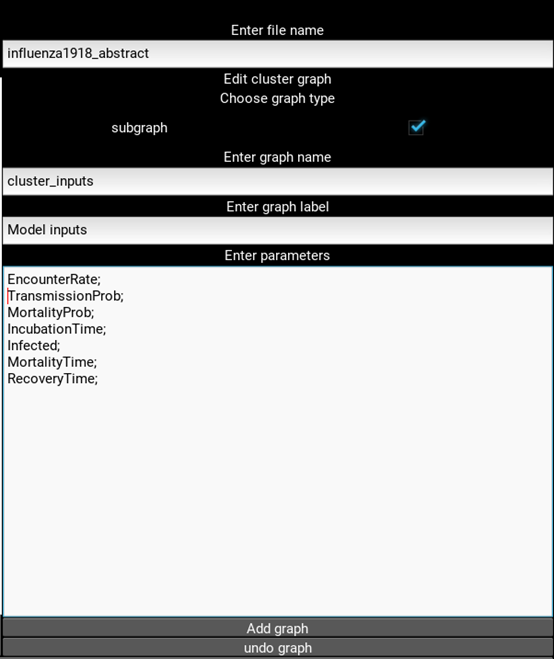
\includegraphics[width=10cm]{figures/influenzaTestProcess3.png}\\
	\caption{Edit graph for input parameters.}
	\label{fig:figure21}
\end{figure}
\noindent 
After added the graph, the left panel will then display the graph via Graphviz. Next is edit the relations between these parameters.
\begin{figure}[H]
	\centering
	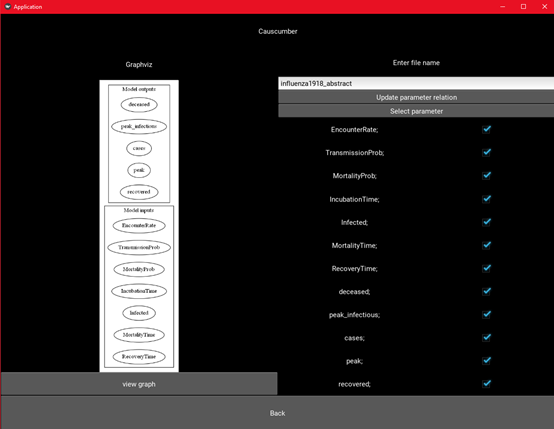
\includegraphics[width=10cm]{figures/influenzaTestProcess5.png}\\
	\caption{Edit relation for parameters.}
	\label{fig:figure23}
\end{figure}
\noindent 
First, select the file, then select the parameters that are going to be affected via the check-boxes, then select the parameters that are going to affect them via the drop-down menu, then the left panel will be updated.
\begin{figure}[H]
	\centering
	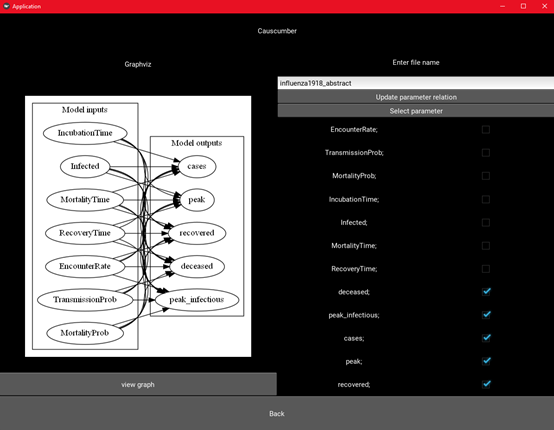
\includegraphics[width=10cm]{figures/influenzaTestProcess7.png}\\
	\caption{Relations of parameters presented in Graphviz graph.}
	\label{fig:figure25}
\end{figure}
\noindent 
After finishing editing the relationship, click back to return to the main menu.
Next user will need to edit the three background files. In environment.py, edit the run\_influenza1918 function to execute the influenza1918 model. Then for dag\_steps.py, define metavariables in the background, a metavariable called “m” needs a function “populate\_m” define. Last is for abstract.py file, apply custom constrain to the parameters of the tested model. \\*\\*
Finally is the \textsl{.feature} file, use “Edit feature files” to create a feature file. Starting from the top user will need to define the feature file’s name, its parameters and its value/distribution and type,
\begin{figure}[H]
	\centering
	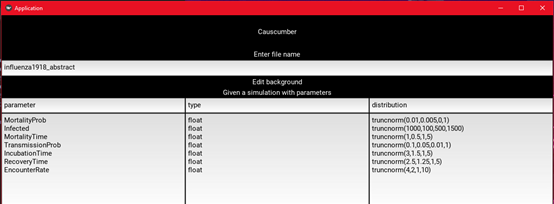
\includegraphics[width=10cm]{figures/influenzaTestProcess10.png}\\
	\caption{Edit initial parameters name, type and value/distribution in influenza1918.}
	\label{fig:figure28}
\end{figure}
\noindent 
Next step is to define what parameter to record and when to record, since influenza1918 doesn’t require any meta variable, that part will be left empty.
\begin{figure}[H]
	\centering
	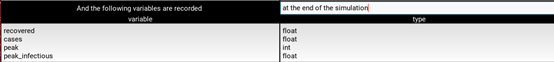
\includegraphics[width=10cm]{figures/influenzaTestProcess11.png}\\
	\caption{Edit recorded parameters name and type in influenza1918.}
	\label{fig:figure29}
\end{figure}
\noindent 
Next is to define the edges for the parameters, this process is same as edit dot file step. Since scenario outline is required in this case, next part will also be skip. Last is scenario, in the right panel, edit the change and expected outcome. 
\begin{figure}[H]
	\centering
	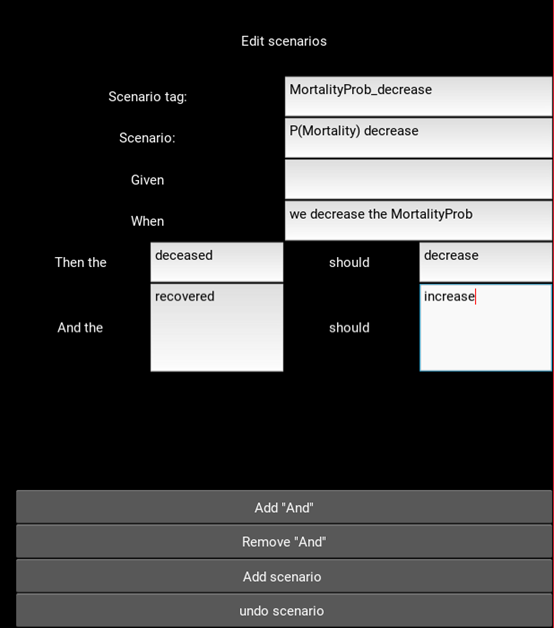
\includegraphics[width=10cm]{figures/influenzaTestProcess12.png}\\
	\caption{Edit scenario for influenza1918.}
	\label{fig:figure30}
\end{figure}
\noindent 
Upon finish edit all the scenario, user can then return to main menu and then select the feature file. After select feature file, user run behave to produce the result on the screen,
\begin{figure}[H]
	\centering
	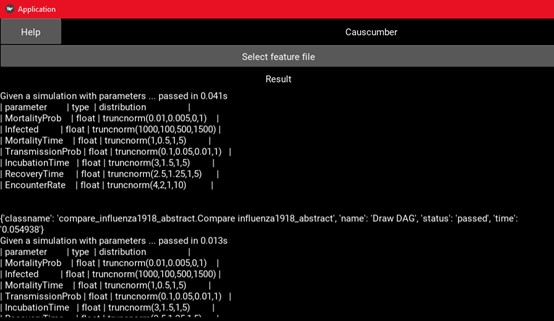
\includegraphics[width=10cm]{figures/influenzaTestProcess15.png}\\
	\caption{Result produced by Causcumber display in result section.}
	\label{fig:figure33}
\end{figure}

\subsection{Testing result for influenza1918}
In the result produced by Causcumber, either with the assisting tool or without, all produce the same result. In the files produced by the tool, starting with \textsl{.dot} file, it is identical with manually created version with some minor difference in formats that doesn’t matter in this case. With this assist of the tool, this process also become a lot more efficient. Next are the three background files, in those files, most of the parts are already pre-define with some parts that can only be manually define by user. Last, in \textsl{.feature} file, the file generated by the tool is no difference compare to the manually created file, and by splitting the files into different sections, and edit it one by one, it become more streamline and readable from a user’s point of view. 
\subsection{Discuss influenza1918 result}
With the assisting tool, creating test for influenza are relatively simplify because as a user, it is not necessary to understand all the syntax for all the files. And with the auto generated files, since not all the parts require manually input, the chance of error occur has been reduced. One of the problem originally user may encounter when define edges for files such as \textsl{.dot} file and \textsl{.feature} file, is that it is difficult for user to list all the edges without any sort of visualization. With the Graphviz’s assist, this process become much clearer during the process. Unfortunately, for the three background files, part of it still require user to manually code those parts in due to the methods used by developers to code computational model maybe drastic different. Overall, this result satisfy the requirement to reduce the need for user to code directly, a more convenient way to create a feature file and Dot file, and with the result being organized into a more clearly displayed format, it also satisfy the making result clean and easy to understand requirement.
\section{Testing Covasim}
Covasim is an agent-based model pf COVID-19 dynamics and interventions, it simulate individual people as an agent, agents will be assigned different states such as infectious or recovered, agents can change to different states and in each states can provide different affects to the simulations. Agents will also be affected by the “Interventions” such as masks or physical distancing. Compare to influenza1918 models in the previous section, this model is a lot more complex with more parameters and methods. 
\subsection{Testing process for Covasim}
First a scenario name “Covasim” is created, in this scenario, in this test, we focus on the interventions part of Covasim. Starting with \textsl{.dot} file, one graph for input parameter and another one for output is created, then the following relations are defined,
\begin{figure}[H]
	\centering
	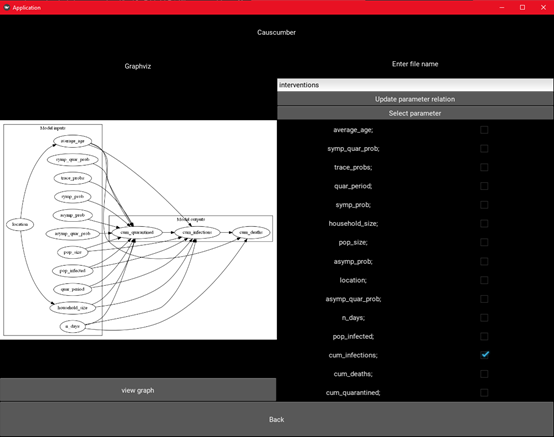
\includegraphics[width=10cm]{figures/CovasimTestProcess2.png}\\
	\caption{Relation for parameters for testing Covasim.}
	\label{fig:figure35}
\end{figure}
\noindent 
Next is to define the three-background file, in \textsl{abstract.py}, there are two custom constraints needs to be define, “average\_age” and “household\_size”. In covasim, one of the parameters requires string, therefore in \textsl{dag\_steps.py} a custom constrain named “countries” is defined. Next, there are several meta variables in the background, these meta variables are also defined as functions in \textsl{dag\_steps.py}. \\*\\*
Last is the feature file, in the first section, one of the parameters is location, since it only accepts string, its distribution will be using the custom distribution “countries” defined before. Also, there are meta variables require, so in this section meta variable are also required to be defined. There is also multiple extra initial condition require to be defined, this is also done in the first section.
\begin{figure}[H]
	\centering
	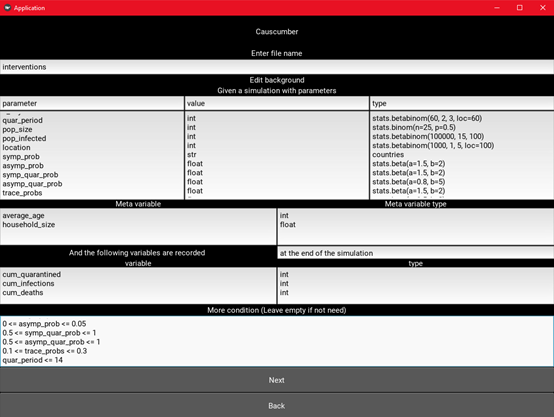
\includegraphics[width=10cm]{figures/CovasimTestProcess3.png}\\
	\caption{Background for testing Covasim.}
	\label{fig:figure36}
\end{figure}
\noindent 
In next section, same as influenza1918, edges are defined using the assisting tools, in Covasim, there are additional edges being added, so instead of choosing next, choose “And add edges” options to add more edges, this is similar function as define edges, but will return slightly different result in the generated feature file. Next, is to edit the scenario outline, by changing the column and row amount, we can provide information according to the requirement of the scenario outline. After this is scenarios, this process is same as influenza1918, with all these steps done, select the newly created feature file, and run Beheve.
\begin{figure}[H]
	\centering
	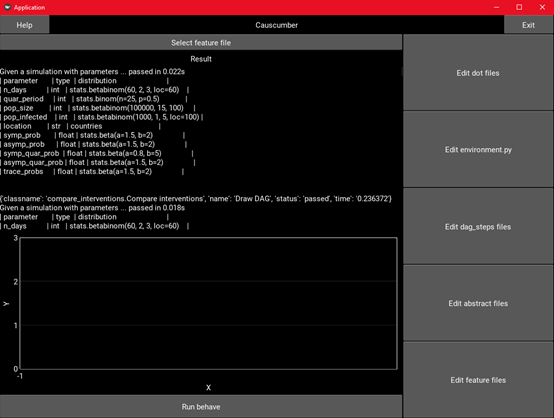
\includegraphics[width=10cm]{figures/CovasimTestProcess6.png}\\
	\caption{Result produced by using assisting tool.}
	\label{fig:figure39}
\end{figure}
\noindent 
\subsection{Testing result for Covasim}
In the testing result for Covasim, result produced by are similar to manually created version, in the manually created version of feature file, some Cucumber syntax can be used to reduce the length of the file, this isn’t replicate the version created by the tool. As for the test result produced by Causcumber, it is mostly identical to the manually created version with some difference in indentation which doesn’t affect the result. When execute the created feature file, user see the displayed result in the result section in an organized format.
\subsection{Discuss Covasim result}
In the testing process for Covasim, the tool provides a lot of assists in the process, especially in the process of defining relation of parameter, and the editing process of feature file. But with the background files, despite the guide provided, it still requires user to have decent programming skill to accomplish it. Overall, with the assist of the tool, the testing process has become more streamline and swift, but parts of the system still holds back by necessity to manually code the test. The result produced by Causcumber is as expected, trimmed are focus on the important parts, which is very useful for user.
\section{A summary of results}
In the result provided by testing on influenza1918, it shows that with the help of the tool, testing become more convenient. The process is overall simplified by reduce the need for user to directly interact with the coding part of testing. With the parts that is necessary for the process, it is mostly reduced by auto generate most of it, with some minor parts still require to be define. This is also the same when defining \textsl{.feature} file, without the need to deal with syntax and format, this process become a lot more smoother. \\*\\*
For covasim, the experience is mostly same when it comes defining relations for parameter and creating feature file, without the need to directly code these files, and with the help of the GUI, the testing process is a lot more understandable and streamline. But when it comes to the background files, despite the auto generated parts, there are still more required to be define. Consider that Covasim is a more complex model, this is to be expected, but this part also shows that if the user tends to add a lot of custom testing aspect, the testing process could still become lengthy.\\*\\*
Combine the information provide by two models, it shows that in terms of editing \textsl{.feature} file and \textsl{.dot} file. This tool can effectively assist user, but when it comes to the background file, if the user is intended to have many custom conditions, then the user will be required to do a decent amount of editing in the background files, this may discourage people to participate in testing.
\section{How does the tool help user simplify the testing process}
As shown by the result, the tool can effectively assist user by allowing user to ignore the required syntax to edit the dot and feature file, with the tool, user will only be required to input the data hinted by the GUI. In this way, user will not be required to learn the complete syntax of the file, make it easier to promote this system to people who aren’t specialize in software testing.\\*\\*
In the files that require manually input, parts of the files will be auto generated. In these files, a total of 319 lines of code will be auto generated, most of it are essential function for the working of Causcumber and will require a decent understanding in Causcumber system to implement those lines. The auto generated parts of the files, together with the assist generated dot and feature file, lowers the skill requirement to use the Causcumber.\\*\\*
To summarize, two main difficulties in using Causcumber are tackled, first is the need to understand the syntax when edit dot and feature file, second is background files for Causcumber. With these two-problem tackled, user won’t necessarily need to understand how Causcumber work, but will only require to know where to input the parameters, which guides are provided to help user in the process. The requirement listed in previous chapter is also satisfied, guides and the overall structure of the interface help user knowing where to start, the need to code directly is generally reduced, user can use the interface to select feature file to test and receive the result in the result section.





